SimHash is one of the methods of LSH, it was proposed to estimate the Angular
metric between two data points. It relies on drawing random lines (from Gaussian
distribution) on the data space and determine the value of the hashing by
observing if the data point is on the positive or negative side of this randomly
drawn line. The positive side indicates a hashing value of 1, and the negative
side indicates a hashing value of 0 (sometimes -1 is used instead).

\begin{figure}[h]
    \centering
    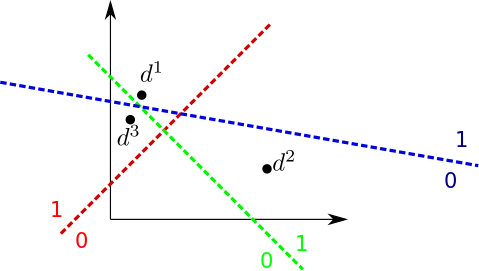
\includegraphics[height=0.28\textheight, width=0.7\textwidth]{state_of_the_art/methods/simhash_lines.png}
    \caption{Simhash LSH illustration}
    \label{fig:simhash_lines}
\end{figure}

The figure \ref{fig:simhash_lines} shows an example on how are the hashing
values determined according to their positions with the randomly drawn lines.

\subsubsection{Formulation}
SimHash method takes $p$ random normalized vectors, and compute the scalar
product of each one of them by the data point's vector $x$ (this will be
identical to the cosine similarity since the vectors are normalized):
$$
    h_p(x_i) = 0 \; \; \; \; if \; \; \; w_i . x_i \leq 0 \; \; ; \; \; h_p(x_i) = 1 \; \; if \; \; w_i . x_i > 0
$$
The collision probability, as shown in section \ref{subsect:angular_metric}
(for one hash), is: $1 -\frac{\theta}{\pi}$. Now, having $p$ hashing functions, it becomes:
$$
    P(H(x_i) = H(x_j) ) = (1 - \frac{\theta}{\pi})
$$

Simhash was one of the first variants of LSH and was widely used in near
duplicate document detection (plagiarism detection for example). The other
variants extended the use to document similarity, image classification and so
on. SimHash gives advantages over MinHash LSH (\ref{subsect:minhash_lsh}) when
it comes to the cases where the data is continuous, in this way, when a couple
of data points is detected similar, it implies that they had a small angle
between them as this method estimates the angles between data points.

It also found use in the classification of users' interests as it was introduced
in Evaluation of Cohort Algorithms for the FLoC API \citep{google_floc_2020}.


\subsubsection{SortingLSH}
This same paper \citep{google_floc_2020} has introduced a new LSH method that
relies on Simhash called SortingLSH.

The intuition behind the SortingLSH algorithm is to sort the hashing vectors
given by the Simhash method, and group them to form clusters. It is a method
that processes over the SimHash clusters, in order to give more control on the
size of each cluster which is an important criteria in the case of Ads to
assure the user's privacy.

Simhash algorithm is formulated given a dataset $D$ of dimension $(n, d)$, we
compute for each data point its hashing vector as in the SimHash method:
$(h_1=H_p (x_1) , h_2=H_p (x_2) ,.., h_n=H_p (x_n))$. Those vectors are sorted
in a \gls{lexicographical} order and then assigned to clusters by generating
contiguous groups of at least $k$ hashes.
